\documentclass[11pt]{article}
\usepackage[hmargin=1.5cm, vmargin=1.5cm]{geometry}
\usepackage{listings}
\usepackage{graphicx}
\graphicspath{{C:/Calculator Project/}}
\begin{document}
\begin{center}
\textbf{Assignment \#07}\\
\textbf{0801CS211088}\\
\vspace{.5cm}
\textbf{\huge Calculator}\\ 
\end{center}
\vspace{.5cm}
\textbf{ \large Project Objective: } \\
This is a simple calulator that can perform various operations on numbers. This program is developed in C++.
\\ \\
\textbf{ \large Statistics: } \\ 
Starting Date: 16/11/2022 \\
End Date: 20/11/2022  \\
Total Days: 5 Days \\
Total Line of Code : 192 \\ \\ \\
\textbf{ \large Functions used: } \\
\textbf{1. add(int num1,int num2:} This function adds two numbers which we need to pass as arguements. \\ 
\textbf{2. sub(int num1,int num):}  This function subtracts two numbers which we need to pass as arguements. \\
\textbf{3. mult(int num1,int num2):} This function multiplies two numbers which we need to pass as arguements. \\
\textbf{4. div(int num1,int num2):} This function divides two numbers which we need to pass as arguements.  \\
\textbf{5. Expcalc(int num1,int num2):} This function caclulates the power of a  number when passesd as arguements. \\
\textbf{6. factorial(int num1):} This function calculates the factorial of the fiirst number which is passes as arguement. \\
\textbf{7. permutation(int num1,int num2):} This function calculates the permutation of two number which we need to pass as arguements. \\
\textbf{8. combination(int num1,int num2):} This function calculates the permutation of two number which we need to pass as arguements. \\
\textbf{9. squareroot(int num1):} This function calculates the square root of the first w=number which is passed as arguement. \\
\pagebreak
\textbf{10. main():} Main function which executes the whole program with the help of switch case.\\
\textbf{\large{Soumya Narvariya}}\hspace{12cm}{\large \textbf{0801CS211088}} \\
\vspace{.5cm}
\rule{18.8cm}{.5mm}  \\
\textbf{\Large Program Code: }\\ \\
\begin{lstlisting}
#include<iostream>
#include<conio.h>
#include<math.h>
using namespace std;

/** 
 * Function declarations for calculator
 */
float add(float num1, float num2);
float sub(float num1, float num2);
float mult(float num1, float num2);
float div(float num1, float num2);
int Expcalc(int num1, int num2);
int factorial(int num1);
int permutation(int num1, int num2);
float squareroot(int num1);
int combination(int num1, int num2);

int main()
{
    for(int j=0;j<50;j++)
    {
    int op;
    float num1, num2, result=0.0f;
    /* Print welcome message */
    cout<<("\nWELCOME TO SIMPLE CALCULATOR\n");
    cout<<("----------------------------\n");
    cout<<("Enter [number 1] [number 2]\n");
    cin>>num1>>num2;
    cout<<"What operation do you want to perform ?"<<endl;
    cout<<"1. Addition"<<endl;
    cout<<"2. Subtraction"<<endl;
    cout<<"3. Multiplication"<<endl;
    cout<<"4. Division"<<endl;
    cout<<"5. Factorial"<<endl;
    cout<<"6. Permutation"<<endl;
    cout<<"7. Combination"<<endl;
    cout<<"8. Exponential power calulation"<<endl;
    cout<<"9. Square roots"<<endl;
    cout<<"10. Exit"<<endl;
    cout<<"Enter your choice: ";
    cin>>op;
    if(op==10)
    {
        break;
    }
    switch(op)
    {
        case 1: 
            result = add(num1, num2);
            break;

        case 2: 
            result = sub(num1, num2);
            break;

        case 3: 
            result = mult(num1, num2);
            break;

        case 4: 
            result = div(num1, num2);
            break;
        case 5:
            result = factorial(num1);
            break;
        case 6:
            result = permutation(num1,num2);
            break;
        case 7:
            result = combination(num1, num2);
            break;
        case 8:
            result = Expcalc(num1, num2);
            break;
        case 9:
            result = squareroot(num1);
            break;
        case 10:
            break;
        default: 
            cout<<"Invalid operatoion"<<endl;
    }
    
    cout<<"Result: "<<result;
    getch();
    }
    return 0;
}

/**
 * Function to add two numbers
 */
float add(float num1, float num2)
{
    return num1 + num2;
}

/**
 * Function to subtract two numbers
 */
float sub(float num1, float num2)
{
    return num1 - num2;
}

/**
 * Function to multiply two numbers
 */
float mult(float num1, float num2)
{
    return num1 * num2;
}

/**
 * Function to divide two numbers
 */
float div(float num1, float num2)
{
    return num1 / num2;
}

/**
 *  Function to find factorial of a number
*/
int factorial(int num1)
{
    int factorial=1;
    for(int i=1;i<=num1;i++)
    {
        factorial=factorial*i;
    }
    return factorial;
}

/**
 *  Function to find Permutation of two numbers
*/
int permutation(int num1, int num2)
{
    int n,r,n_factorial=1,nr_factorial=1;
    n=max(num1,num2);
    r=min(num1,num2);
    for(int i=1;i<=n;i++)
    {
        n_factorial=n_factorial*i;
    }
    for(int i=1;i<=(n-r);i++)
    {
        nr_factorial=nr_factorial*i;
    }
    return n_factorial/nr_factorial;
}

/**
 * Function to find Combination of two numbers
*/
int combination(int num1, int num2)
{
     int n,r,n_factorial=1,nr_factorial=1,r_factorial=1;
    n=max(num1,num2);
    r=min(num1,num2);
    for(int i=1;i<=n;i++)
    {
        n_factorial=n_factorial*i;
    }
    for(int i=1;i<=(n-r);i++)
    {
        nr_factorial=nr_factorial*i;
    }
    for(int i=1;i<=r;i++)
    {
        r_factorial=r_factorial*i;
    }
    return n_factorial/(nr_factorial*r_factorial);
}

/**
 * Function to calculate power of a number
*/
int Expcalc(int num1, int num2)
{
    return pow(num1,num2);
}

/**
 * Function to calulate square root of a number
*/
float squareroot(int num1)
{
    return sqrt(num1);
}
\end{lstlisting}
\pagebreak
\textbf{\large{Soumya Narvariya}}\hspace{12cm}{\large \textbf{0801CS211088}} \\
\vspace{.5cm}
\rule{18.8cm}{.5mm}  \\
\textbf{\Large Debugging: }\\ \\
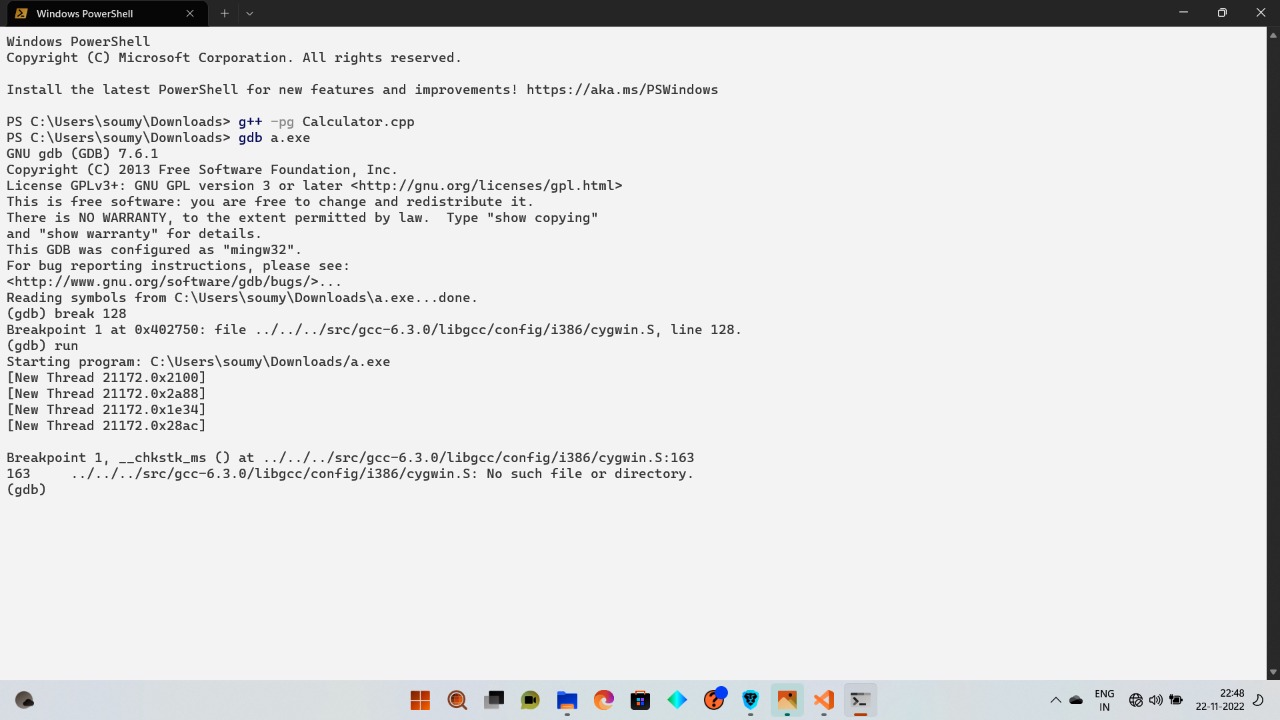
\includegraphics[scale=0.4]{debug1.png}\\ \\
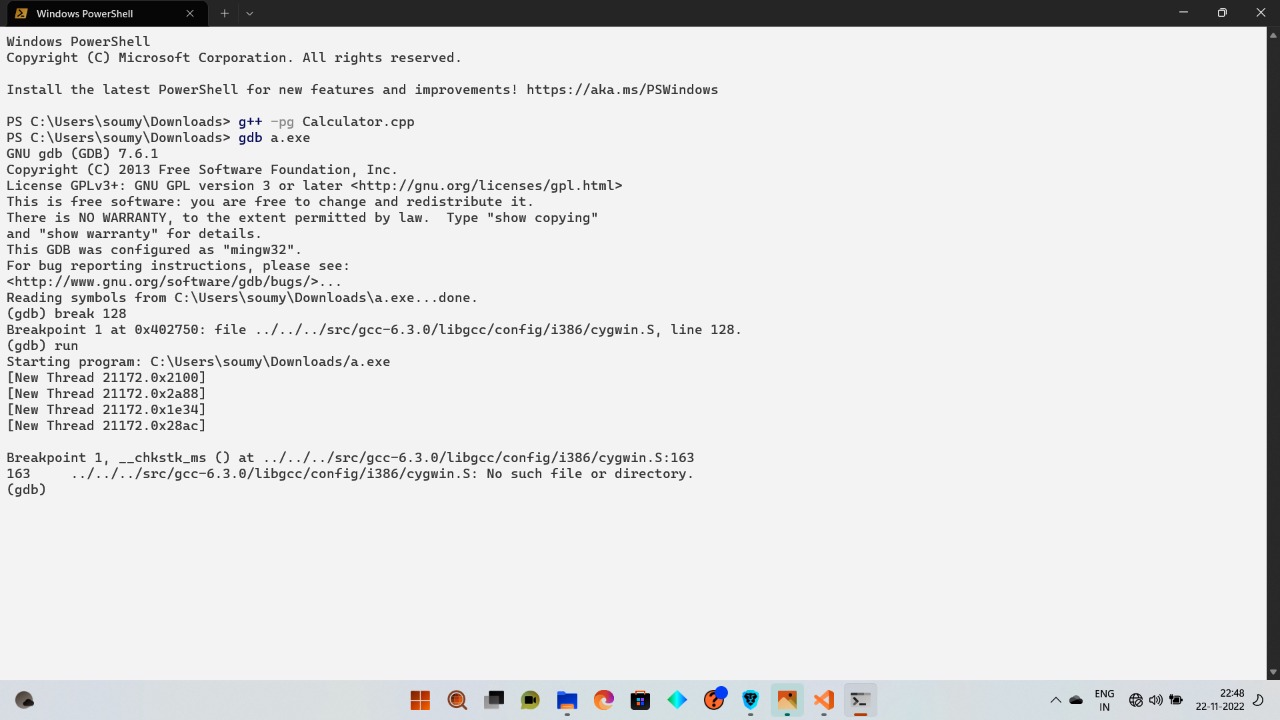
\includegraphics[scale=0.4]{debug2.png}\\ \\
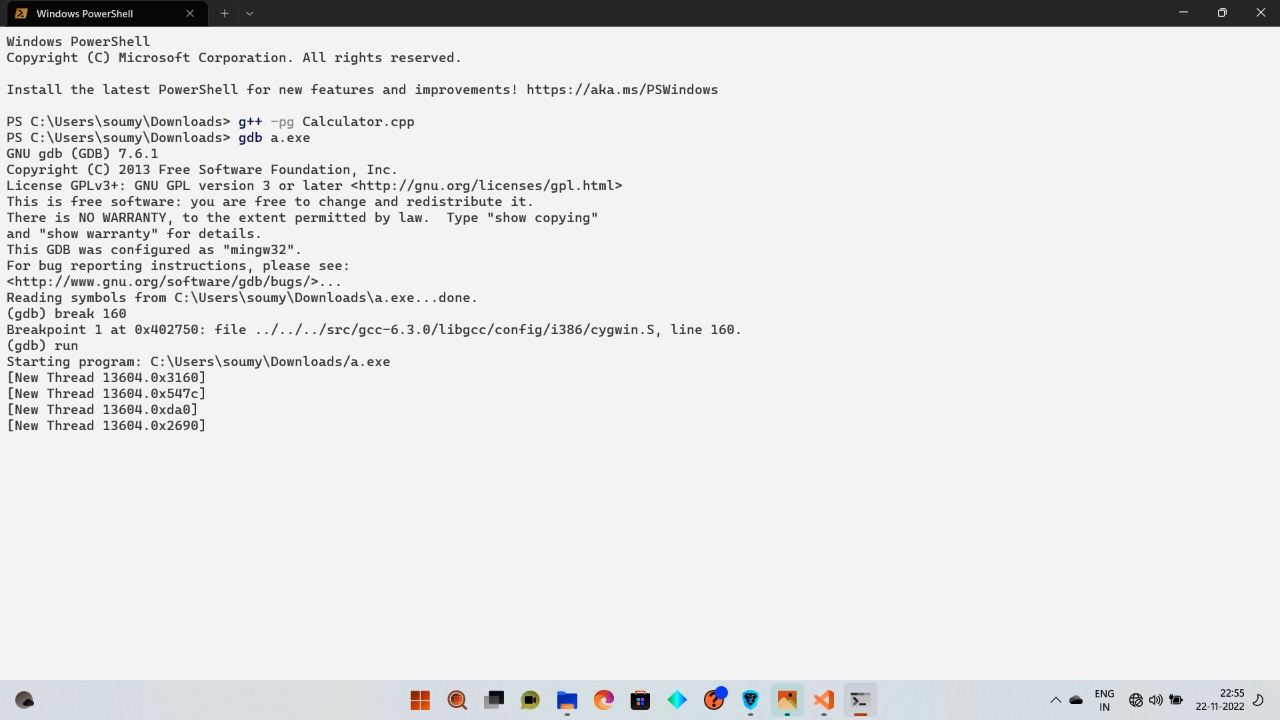
\includegraphics[scale=0.4]{debug3.png}\\ \\
\pagebreak
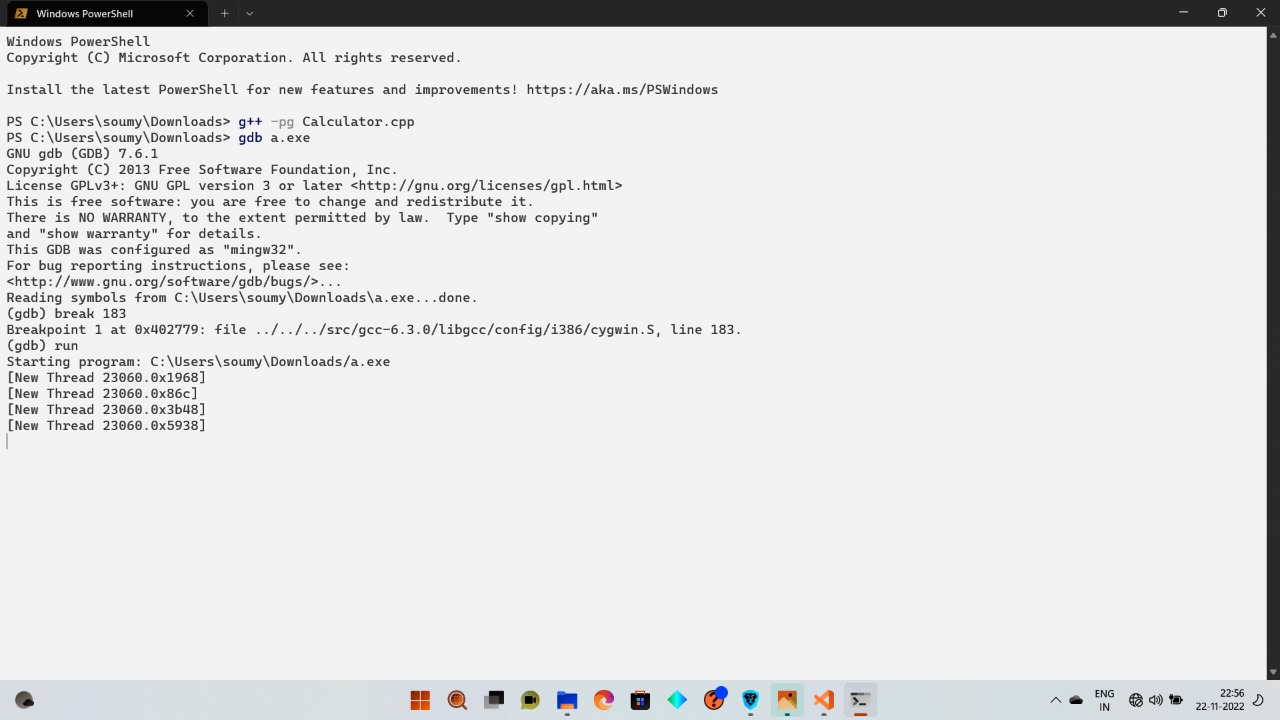
\includegraphics[scale=0.4]{debug4.png}\\ \\
\textbf{\large{Soumya Narvariya}}\hspace{12cm}{\large \textbf{0801CS211088}} \\
\vspace{.5cm}
\rule{18.8cm}{.5mm}  \\
\textbf{\Large Profiling: }\\ \\
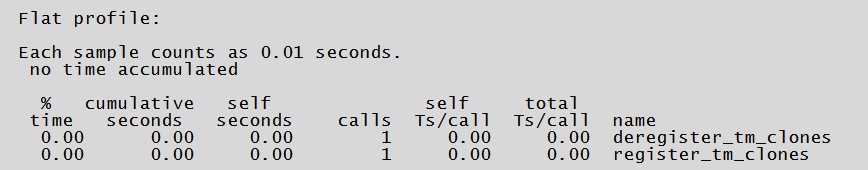
\includegraphics[scale=0.5]{pro1.png}\\ \\
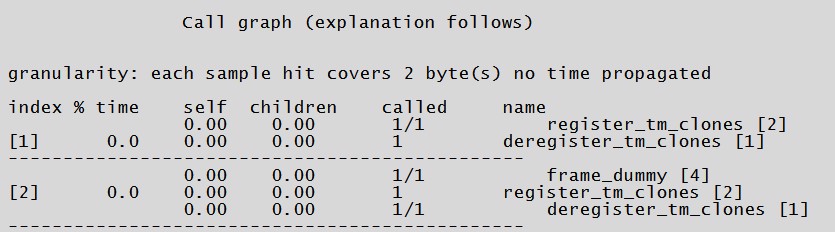
\includegraphics[scale=0.5]{pro2.png}\\ \\
\pagebreak
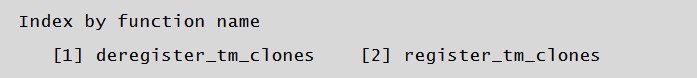
\includegraphics[scale=0.5]{pro3.png}\\ \\
\textbf{\large{Soumya Narvariya}}\hspace{12cm}{\large \textbf{0801CS211088}} \\
\vspace{.5cm}
\rule{18.8cm}{.5mm}  \\
\textbf{\Large Program Output: }\\ \\
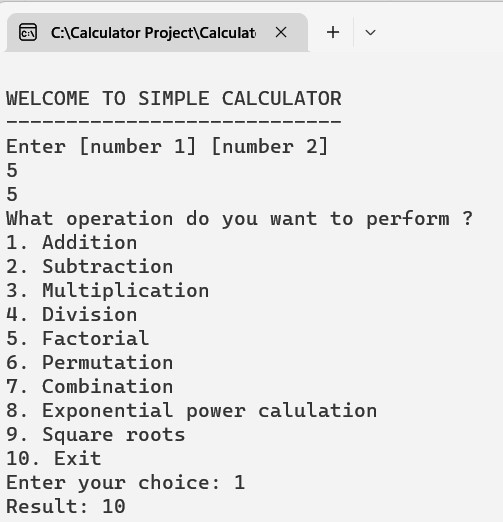
\includegraphics[scale=0.5]{out1.png}\\ \\
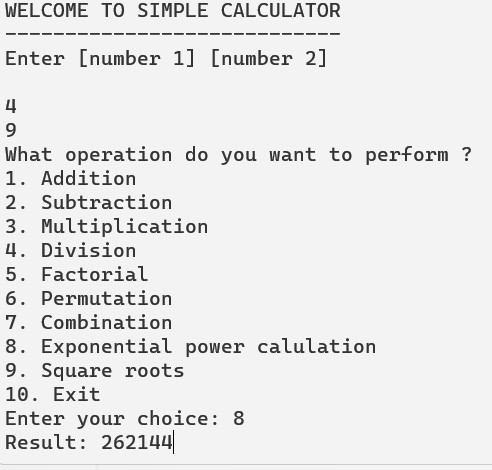
\includegraphics[scale=0.5]{out2.png}\\ \\
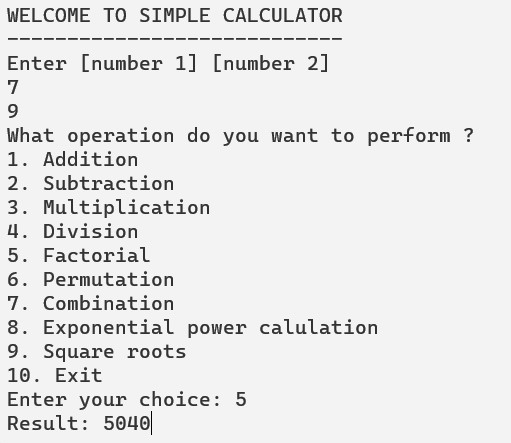
\includegraphics[scale=0.5]{out3.png}\\ \\
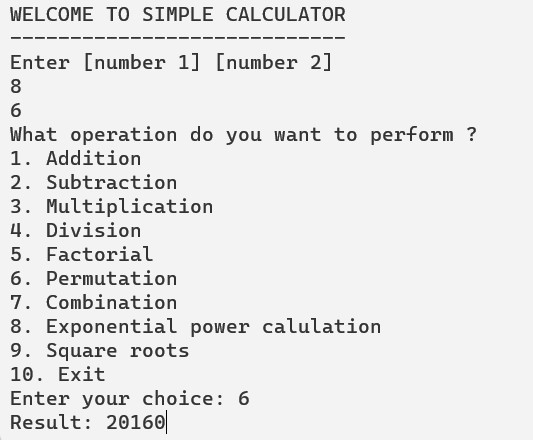
\includegraphics[scale=0.5]{out4.png}\\ \\
\end{document}